% Created by tikzDevice version 0.12.3.1 on 2022-04-28 13:47:58
% !TEX encoding = UTF-8 Unicode
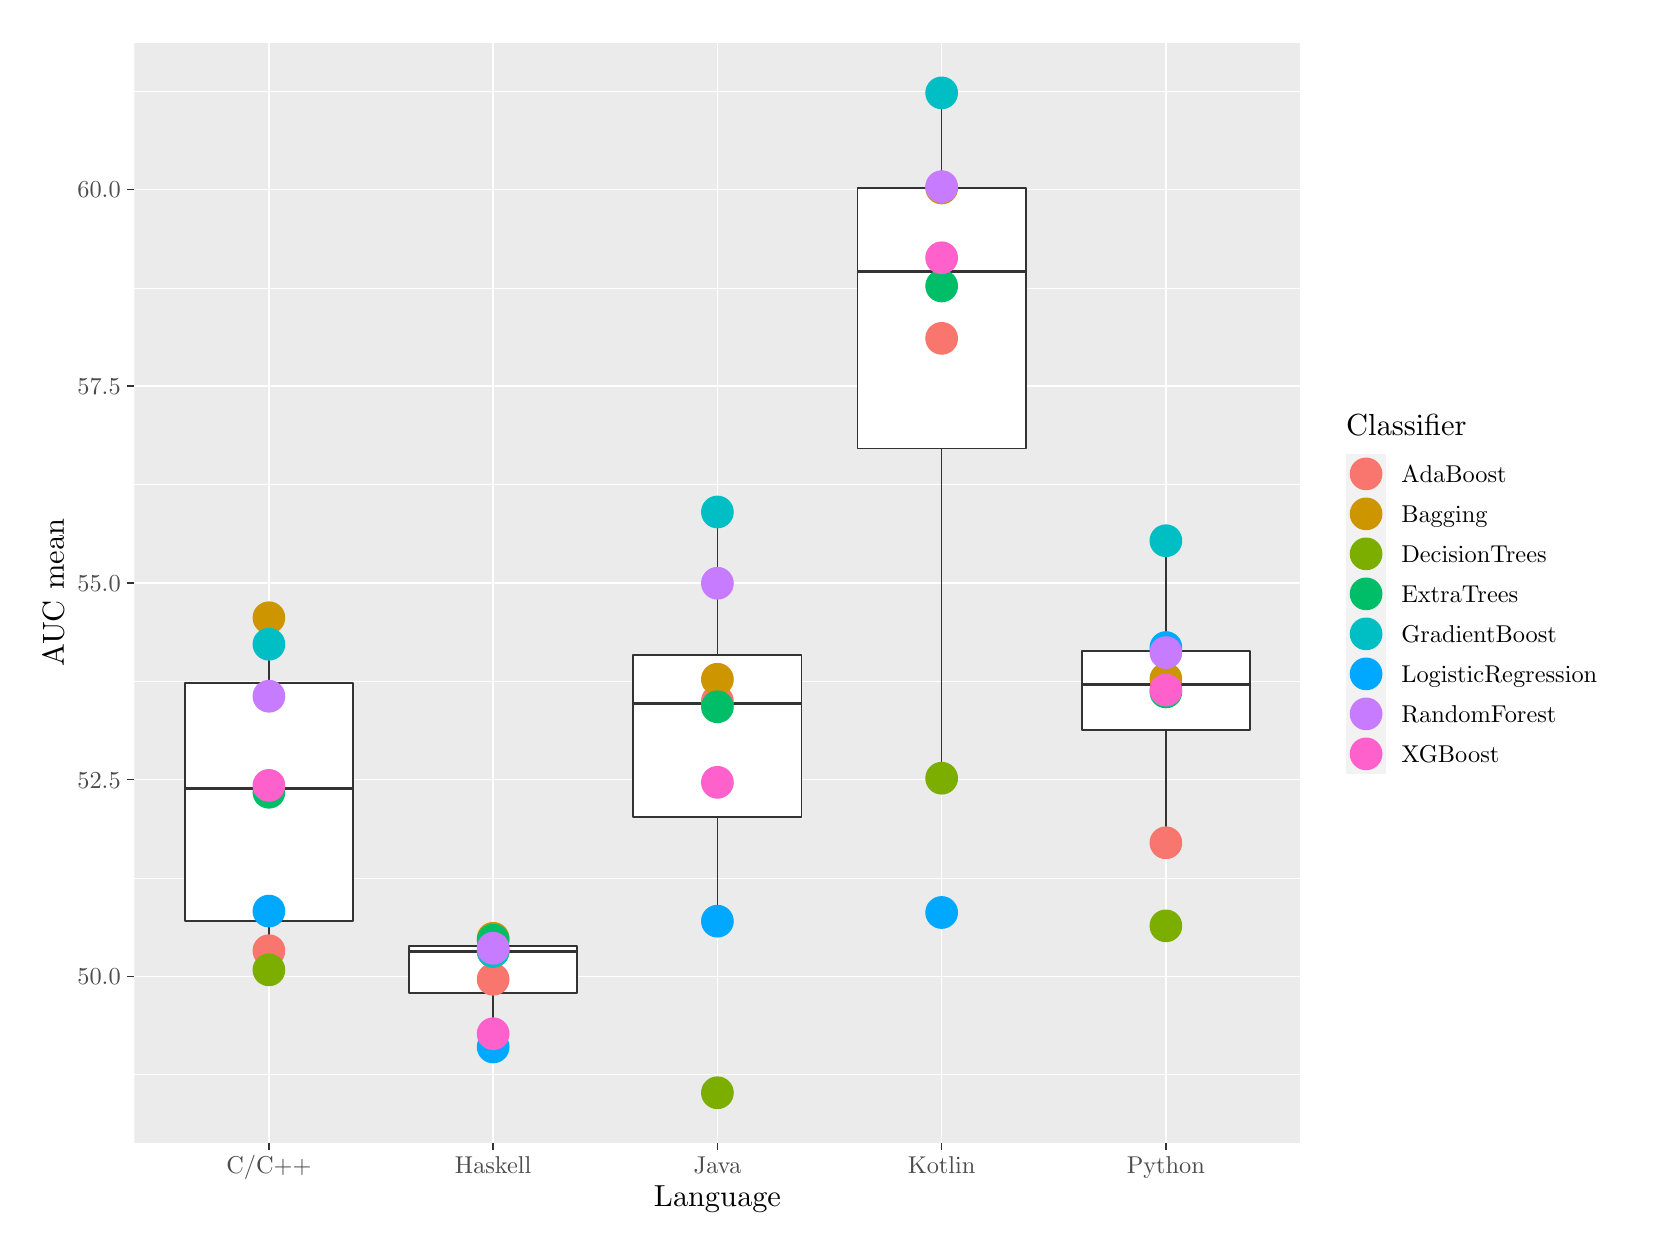
\begin{tikzpicture}[x=1pt,y=1pt]
\definecolor{fillColor}{RGB}{255,255,255}
\path[use as bounding box,fill=fillColor,fill opacity=0.00] (0,0) rectangle (578.16,433.62);
\begin{scope}
\path[clip] (  0.00,  0.00) rectangle (578.16,433.62);
\definecolor{drawColor}{RGB}{255,255,255}
\definecolor{fillColor}{RGB}{255,255,255}

\path[draw=drawColor,line width= 0.6pt,line join=round,line cap=round,fill=fillColor] (  0.00,  0.00) rectangle (578.16,433.62);
\end{scope}
\begin{scope}
\path[clip] ( 38.56, 30.69) rectangle (459.91,428.12);
\definecolor{fillColor}{gray}{0.92}

\path[fill=fillColor] ( 38.56, 30.69) rectangle (459.91,428.12);
\definecolor{drawColor}{RGB}{255,255,255}

\path[draw=drawColor,line width= 0.3pt,line join=round] ( 38.56, 55.29) --
	(459.91, 55.29);

\path[draw=drawColor,line width= 0.3pt,line join=round] ( 38.56,126.36) --
	(459.91,126.36);

\path[draw=drawColor,line width= 0.3pt,line join=round] ( 38.56,197.43) --
	(459.91,197.43);

\path[draw=drawColor,line width= 0.3pt,line join=round] ( 38.56,268.50) --
	(459.91,268.50);

\path[draw=drawColor,line width= 0.3pt,line join=round] ( 38.56,339.57) --
	(459.91,339.57);

\path[draw=drawColor,line width= 0.3pt,line join=round] ( 38.56,410.64) --
	(459.91,410.64);

\path[draw=drawColor,line width= 0.6pt,line join=round] ( 38.56, 90.82) --
	(459.91, 90.82);

\path[draw=drawColor,line width= 0.6pt,line join=round] ( 38.56,161.89) --
	(459.91,161.89);

\path[draw=drawColor,line width= 0.6pt,line join=round] ( 38.56,232.97) --
	(459.91,232.97);

\path[draw=drawColor,line width= 0.6pt,line join=round] ( 38.56,304.04) --
	(459.91,304.04);

\path[draw=drawColor,line width= 0.6pt,line join=round] ( 38.56,375.11) --
	(459.91,375.11);

\path[draw=drawColor,line width= 0.6pt,line join=round] ( 87.17, 30.69) --
	( 87.17,428.12);

\path[draw=drawColor,line width= 0.6pt,line join=round] (168.20, 30.69) --
	(168.20,428.12);

\path[draw=drawColor,line width= 0.6pt,line join=round] (249.23, 30.69) --
	(249.23,428.12);

\path[draw=drawColor,line width= 0.6pt,line join=round] (330.26, 30.69) --
	(330.26,428.12);

\path[draw=drawColor,line width= 0.6pt,line join=round] (411.29, 30.69) --
	(411.29,428.12);
\definecolor{drawColor}{gray}{0.20}

\path[draw=drawColor,line width= 0.6pt,line join=round] ( 87.17,196.73) -- ( 87.17,220.39);

\path[draw=drawColor,line width= 0.6pt,line join=round] ( 87.17,110.82) -- ( 87.17, 93.16);
\definecolor{fillColor}{RGB}{255,255,255}

\path[draw=drawColor,line width= 0.6pt,line join=round,line cap=round,fill=fillColor] ( 56.79,196.73) --
	( 56.79,110.82) --
	(117.56,110.82) --
	(117.56,196.73) --
	( 56.79,196.73) --
	cycle;

\path[draw=drawColor,line width= 1.1pt,line join=round] ( 56.79,158.57) -- (117.56,158.57);

\path[draw=drawColor,line width= 0.6pt,line join=round] (168.20,101.71) -- (168.20,104.57);

\path[draw=drawColor,line width= 0.6pt,line join=round] (168.20, 84.84) -- (168.20, 65.30);

\path[draw=drawColor,line width= 0.6pt,line join=round,line cap=round,fill=fillColor] (137.82,101.71) --
	(137.82, 84.84) --
	(198.59, 84.84) --
	(198.59,101.71) --
	(137.82,101.71) --
	cycle;

\path[draw=drawColor,line width= 1.1pt,line join=round] (137.82, 99.87) -- (198.59, 99.87);
\definecolor{fillColor}{gray}{0.20}

\path[draw=drawColor,line width= 0.4pt,line join=round,line cap=round,fill=fillColor] (249.23, 48.75) circle (  1.96);

\path[draw=drawColor,line width= 0.6pt,line join=round] (249.23,206.83) -- (249.23,258.61);

\path[draw=drawColor,line width= 0.6pt,line join=round] (249.23,148.38) -- (249.23,110.75);
\definecolor{fillColor}{RGB}{255,255,255}

\path[draw=drawColor,line width= 0.6pt,line join=round,line cap=round,fill=fillColor] (218.85,206.83) --
	(218.85,148.38) --
	(279.62,148.38) --
	(279.62,206.83) --
	(218.85,206.83) --
	cycle;

\path[draw=drawColor,line width= 1.1pt,line join=round] (218.85,189.26) -- (279.62,189.26);
\definecolor{fillColor}{gray}{0.20}

\path[draw=drawColor,line width= 0.4pt,line join=round,line cap=round,fill=fillColor] (330.26,113.89) circle (  1.96);

\path[draw=drawColor,line width= 0.6pt,line join=round] (330.26,375.80) -- (330.26,410.05);

\path[draw=drawColor,line width= 0.6pt,line join=round] (330.26,281.61) -- (330.26,162.41);
\definecolor{fillColor}{RGB}{255,255,255}

\path[draw=drawColor,line width= 0.6pt,line join=round,line cap=round,fill=fillColor] (299.87,375.80) --
	(299.87,281.61) --
	(360.65,281.61) --
	(360.65,375.80) --
	(299.87,375.80) --
	cycle;

\path[draw=drawColor,line width= 1.1pt,line join=round] (299.87,345.37) -- (360.65,345.37);
\definecolor{fillColor}{gray}{0.20}

\path[draw=drawColor,line width= 0.4pt,line join=round,line cap=round,fill=fillColor] (411.29,109.06) circle (  1.96);

\path[draw=drawColor,line width= 0.6pt,line join=round] (411.29,208.26) -- (411.29,248.22);

\path[draw=drawColor,line width= 0.6pt,line join=round] (411.29,179.95) -- (411.29,139.08);
\definecolor{fillColor}{RGB}{255,255,255}

\path[draw=drawColor,line width= 0.6pt,line join=round,line cap=round,fill=fillColor] (380.90,208.26) --
	(380.90,179.95) --
	(441.68,179.95) --
	(441.68,208.26) --
	(380.90,208.26) --
	cycle;

\path[draw=drawColor,line width= 1.1pt,line join=round] (380.90,196.27) -- (441.68,196.27);
\definecolor{drawColor}{RGB}{248,118,109}
\definecolor{fillColor}{RGB}{248,118,109}

\path[draw=drawColor,line width= 0.4pt,line join=round,line cap=round,fill=fillColor] ( 87.17,100.08) circle (  5.71);
\definecolor{drawColor}{RGB}{205,150,0}
\definecolor{fillColor}{RGB}{205,150,0}

\path[draw=drawColor,line width= 0.4pt,line join=round,line cap=round,fill=fillColor] ( 87.17,220.39) circle (  5.71);
\definecolor{drawColor}{RGB}{124,174,0}
\definecolor{fillColor}{RGB}{124,174,0}

\path[draw=drawColor,line width= 0.4pt,line join=round,line cap=round,fill=fillColor] ( 87.17, 93.16) circle (  5.71);
\definecolor{drawColor}{RGB}{0,190,103}
\definecolor{fillColor}{RGB}{0,190,103}

\path[draw=drawColor,line width= 0.4pt,line join=round,line cap=round,fill=fillColor] ( 87.17,157.33) circle (  5.71);
\definecolor{drawColor}{RGB}{0,191,196}
\definecolor{fillColor}{RGB}{0,191,196}

\path[draw=drawColor,line width= 0.4pt,line join=round,line cap=round,fill=fillColor] ( 87.17,210.82) circle (  5.71);
\definecolor{drawColor}{RGB}{0,169,255}
\definecolor{fillColor}{RGB}{0,169,255}

\path[draw=drawColor,line width= 0.4pt,line join=round,line cap=round,fill=fillColor] ( 87.17,114.40) circle (  5.71);
\definecolor{drawColor}{RGB}{199,124,255}
\definecolor{fillColor}{RGB}{199,124,255}

\path[draw=drawColor,line width= 0.4pt,line join=round,line cap=round,fill=fillColor] ( 87.17,192.03) circle (  5.71);
\definecolor{drawColor}{RGB}{255,97,204}
\definecolor{fillColor}{RGB}{255,97,204}

\path[draw=drawColor,line width= 0.4pt,line join=round,line cap=round,fill=fillColor] ( 87.17,159.81) circle (  5.71);
\definecolor{drawColor}{RGB}{248,118,109}
\definecolor{fillColor}{RGB}{248,118,109}

\path[draw=drawColor,line width= 0.4pt,line join=round,line cap=round,fill=fillColor] (168.20, 89.75) circle (  5.71);
\definecolor{drawColor}{RGB}{205,150,0}
\definecolor{fillColor}{RGB}{205,150,0}

\path[draw=drawColor,line width= 0.4pt,line join=round,line cap=round,fill=fillColor] (168.20,104.57) circle (  5.71);
\definecolor{drawColor}{RGB}{124,174,0}
\definecolor{fillColor}{RGB}{124,174,0}

\path[draw=drawColor,line width= 0.4pt,line join=round,line cap=round,fill=fillColor] (168.20, 99.82) circle (  5.71);
\definecolor{drawColor}{RGB}{0,190,103}
\definecolor{fillColor}{RGB}{0,190,103}

\path[draw=drawColor,line width= 0.4pt,line join=round,line cap=round,fill=fillColor] (168.20,103.93) circle (  5.71);
\definecolor{drawColor}{RGB}{0,191,196}
\definecolor{fillColor}{RGB}{0,191,196}

\path[draw=drawColor,line width= 0.4pt,line join=round,line cap=round,fill=fillColor] (168.20, 99.92) circle (  5.71);
\definecolor{drawColor}{RGB}{0,169,255}
\definecolor{fillColor}{RGB}{0,169,255}

\path[draw=drawColor,line width= 0.4pt,line join=round,line cap=round,fill=fillColor] (168.20, 65.30) circle (  5.71);
\definecolor{drawColor}{RGB}{199,124,255}
\definecolor{fillColor}{RGB}{199,124,255}

\path[draw=drawColor,line width= 0.4pt,line join=round,line cap=round,fill=fillColor] (168.20,100.97) circle (  5.71);
\definecolor{drawColor}{RGB}{255,97,204}
\definecolor{fillColor}{RGB}{255,97,204}

\path[draw=drawColor,line width= 0.4pt,line join=round,line cap=round,fill=fillColor] (168.20, 70.08) circle (  5.71);
\definecolor{drawColor}{RGB}{248,118,109}
\definecolor{fillColor}{RGB}{248,118,109}

\path[draw=drawColor,line width= 0.4pt,line join=round,line cap=round,fill=fillColor] (249.23,190.30) circle (  5.71);
\definecolor{drawColor}{RGB}{205,150,0}
\definecolor{fillColor}{RGB}{205,150,0}

\path[draw=drawColor,line width= 0.4pt,line join=round,line cap=round,fill=fillColor] (249.23,198.16) circle (  5.71);
\definecolor{drawColor}{RGB}{124,174,0}
\definecolor{fillColor}{RGB}{124,174,0}

\path[draw=drawColor,line width= 0.4pt,line join=round,line cap=round,fill=fillColor] (249.23, 48.75) circle (  5.71);
\definecolor{drawColor}{RGB}{0,190,103}
\definecolor{fillColor}{RGB}{0,190,103}

\path[draw=drawColor,line width= 0.4pt,line join=round,line cap=round,fill=fillColor] (249.23,188.22) circle (  5.71);
\definecolor{drawColor}{RGB}{0,191,196}
\definecolor{fillColor}{RGB}{0,191,196}

\path[draw=drawColor,line width= 0.4pt,line join=round,line cap=round,fill=fillColor] (249.23,258.61) circle (  5.71);
\definecolor{drawColor}{RGB}{0,169,255}
\definecolor{fillColor}{RGB}{0,169,255}

\path[draw=drawColor,line width= 0.4pt,line join=round,line cap=round,fill=fillColor] (249.23,110.75) circle (  5.71);
\definecolor{drawColor}{RGB}{199,124,255}
\definecolor{fillColor}{RGB}{199,124,255}

\path[draw=drawColor,line width= 0.4pt,line join=round,line cap=round,fill=fillColor] (249.23,232.85) circle (  5.71);
\definecolor{drawColor}{RGB}{255,97,204}
\definecolor{fillColor}{RGB}{255,97,204}

\path[draw=drawColor,line width= 0.4pt,line join=round,line cap=round,fill=fillColor] (249.23,160.92) circle (  5.71);
\definecolor{drawColor}{RGB}{248,118,109}
\definecolor{fillColor}{RGB}{248,118,109}

\path[draw=drawColor,line width= 0.4pt,line join=round,line cap=round,fill=fillColor] (330.26,321.35) circle (  5.71);
\definecolor{drawColor}{RGB}{205,150,0}
\definecolor{fillColor}{RGB}{205,150,0}

\path[draw=drawColor,line width= 0.4pt,line join=round,line cap=round,fill=fillColor] (330.26,375.68) circle (  5.71);
\definecolor{drawColor}{RGB}{124,174,0}
\definecolor{fillColor}{RGB}{124,174,0}

\path[draw=drawColor,line width= 0.4pt,line join=round,line cap=round,fill=fillColor] (330.26,162.41) circle (  5.71);
\definecolor{drawColor}{RGB}{0,190,103}
\definecolor{fillColor}{RGB}{0,190,103}

\path[draw=drawColor,line width= 0.4pt,line join=round,line cap=round,fill=fillColor] (330.26,340.28) circle (  5.71);
\definecolor{drawColor}{RGB}{0,191,196}
\definecolor{fillColor}{RGB}{0,191,196}

\path[draw=drawColor,line width= 0.4pt,line join=round,line cap=round,fill=fillColor] (330.26,410.05) circle (  5.71);
\definecolor{drawColor}{RGB}{0,169,255}
\definecolor{fillColor}{RGB}{0,169,255}

\path[draw=drawColor,line width= 0.4pt,line join=round,line cap=round,fill=fillColor] (330.26,113.89) circle (  5.71);
\definecolor{drawColor}{RGB}{199,124,255}
\definecolor{fillColor}{RGB}{199,124,255}

\path[draw=drawColor,line width= 0.4pt,line join=round,line cap=round,fill=fillColor] (330.26,376.17) circle (  5.71);
\definecolor{drawColor}{RGB}{255,97,204}
\definecolor{fillColor}{RGB}{255,97,204}

\path[draw=drawColor,line width= 0.4pt,line join=round,line cap=round,fill=fillColor] (330.26,350.47) circle (  5.71);
\definecolor{drawColor}{RGB}{248,118,109}
\definecolor{fillColor}{RGB}{248,118,109}

\path[draw=drawColor,line width= 0.4pt,line join=round,line cap=round,fill=fillColor] (411.29,139.08) circle (  5.71);
\definecolor{drawColor}{RGB}{205,150,0}
\definecolor{fillColor}{RGB}{205,150,0}

\path[draw=drawColor,line width= 0.4pt,line join=round,line cap=round,fill=fillColor] (411.29,198.28) circle (  5.71);
\definecolor{drawColor}{RGB}{124,174,0}
\definecolor{fillColor}{RGB}{124,174,0}

\path[draw=drawColor,line width= 0.4pt,line join=round,line cap=round,fill=fillColor] (411.29,109.06) circle (  5.71);
\definecolor{drawColor}{RGB}{0,190,103}
\definecolor{fillColor}{RGB}{0,190,103}

\path[draw=drawColor,line width= 0.4pt,line join=round,line cap=round,fill=fillColor] (411.29,193.58) circle (  5.71);
\definecolor{drawColor}{RGB}{0,191,196}
\definecolor{fillColor}{RGB}{0,191,196}

\path[draw=drawColor,line width= 0.4pt,line join=round,line cap=round,fill=fillColor] (411.29,248.22) circle (  5.71);
\definecolor{drawColor}{RGB}{0,169,255}
\definecolor{fillColor}{RGB}{0,169,255}

\path[draw=drawColor,line width= 0.4pt,line join=round,line cap=round,fill=fillColor] (411.29,209.62) circle (  5.71);
\definecolor{drawColor}{RGB}{199,124,255}
\definecolor{fillColor}{RGB}{199,124,255}

\path[draw=drawColor,line width= 0.4pt,line join=round,line cap=round,fill=fillColor] (411.29,207.80) circle (  5.71);
\definecolor{drawColor}{RGB}{255,97,204}
\definecolor{fillColor}{RGB}{255,97,204}

\path[draw=drawColor,line width= 0.4pt,line join=round,line cap=round,fill=fillColor] (411.29,194.26) circle (  5.71);
\end{scope}
\begin{scope}
\path[clip] (  0.00,  0.00) rectangle (578.16,433.62);
\definecolor{drawColor}{gray}{0.30}

\node[text=drawColor,anchor=base east,inner sep=0pt, outer sep=0pt, scale=  0.88] at ( 33.61, 87.79) {50.0};

\node[text=drawColor,anchor=base east,inner sep=0pt, outer sep=0pt, scale=  0.88] at ( 33.61,158.86) {52.5};

\node[text=drawColor,anchor=base east,inner sep=0pt, outer sep=0pt, scale=  0.88] at ( 33.61,229.94) {55.0};

\node[text=drawColor,anchor=base east,inner sep=0pt, outer sep=0pt, scale=  0.88] at ( 33.61,301.01) {57.5};

\node[text=drawColor,anchor=base east,inner sep=0pt, outer sep=0pt, scale=  0.88] at ( 33.61,372.08) {60.0};
\end{scope}
\begin{scope}
\path[clip] (  0.00,  0.00) rectangle (578.16,433.62);
\definecolor{drawColor}{gray}{0.20}

\path[draw=drawColor,line width= 0.6pt,line join=round] ( 35.81, 90.82) --
	( 38.56, 90.82);

\path[draw=drawColor,line width= 0.6pt,line join=round] ( 35.81,161.89) --
	( 38.56,161.89);

\path[draw=drawColor,line width= 0.6pt,line join=round] ( 35.81,232.97) --
	( 38.56,232.97);

\path[draw=drawColor,line width= 0.6pt,line join=round] ( 35.81,304.04) --
	( 38.56,304.04);

\path[draw=drawColor,line width= 0.6pt,line join=round] ( 35.81,375.11) --
	( 38.56,375.11);
\end{scope}
\begin{scope}
\path[clip] (  0.00,  0.00) rectangle (578.16,433.62);
\definecolor{drawColor}{gray}{0.20}

\path[draw=drawColor,line width= 0.6pt,line join=round] ( 87.17, 27.94) --
	( 87.17, 30.69);

\path[draw=drawColor,line width= 0.6pt,line join=round] (168.20, 27.94) --
	(168.20, 30.69);

\path[draw=drawColor,line width= 0.6pt,line join=round] (249.23, 27.94) --
	(249.23, 30.69);

\path[draw=drawColor,line width= 0.6pt,line join=round] (330.26, 27.94) --
	(330.26, 30.69);

\path[draw=drawColor,line width= 0.6pt,line join=round] (411.29, 27.94) --
	(411.29, 30.69);
\end{scope}
\begin{scope}
\path[clip] (  0.00,  0.00) rectangle (578.16,433.62);
\definecolor{drawColor}{gray}{0.30}

\node[text=drawColor,anchor=base,inner sep=0pt, outer sep=0pt, scale=  0.88] at ( 87.17, 19.68) {C/C++};

\node[text=drawColor,anchor=base,inner sep=0pt, outer sep=0pt, scale=  0.88] at (168.20, 19.68) {Haskell};

\node[text=drawColor,anchor=base,inner sep=0pt, outer sep=0pt, scale=  0.88] at (249.23, 19.68) {Java};

\node[text=drawColor,anchor=base,inner sep=0pt, outer sep=0pt, scale=  0.88] at (330.26, 19.68) {Kotlin};

\node[text=drawColor,anchor=base,inner sep=0pt, outer sep=0pt, scale=  0.88] at (411.29, 19.68) {Python};
\end{scope}
\begin{scope}
\path[clip] (  0.00,  0.00) rectangle (578.16,433.62);
\definecolor{drawColor}{RGB}{0,0,0}

\node[text=drawColor,anchor=base,inner sep=0pt, outer sep=0pt, scale=  1.10] at (249.23,  7.64) {Language};
\end{scope}
\begin{scope}
\path[clip] (  0.00,  0.00) rectangle (578.16,433.62);
\definecolor{drawColor}{RGB}{0,0,0}

\node[text=drawColor,rotate= 90.00,anchor=base,inner sep=0pt, outer sep=0pt, scale=  1.10] at ( 13.08,229.40) {AUC mean};
\end{scope}
\begin{scope}
\path[clip] (  0.00,  0.00) rectangle (578.16,433.62);
\definecolor{fillColor}{RGB}{255,255,255}

\path[fill=fillColor] (470.91,158.48) rectangle (572.66,300.33);
\end{scope}
\begin{scope}
\path[clip] (  0.00,  0.00) rectangle (578.16,433.62);
\definecolor{drawColor}{RGB}{0,0,0}

\node[text=drawColor,anchor=base west,inner sep=0pt, outer sep=0pt, scale=  1.10] at (476.41,286.18) {Classifier};
\end{scope}
\begin{scope}
\path[clip] (  0.00,  0.00) rectangle (578.16,433.62);
\definecolor{fillColor}{gray}{0.95}

\path[fill=fillColor] (476.41,265.16) rectangle (490.86,279.61);
\end{scope}
\begin{scope}
\path[clip] (  0.00,  0.00) rectangle (578.16,433.62);
\definecolor{drawColor}{RGB}{248,118,109}
\definecolor{fillColor}{RGB}{248,118,109}

\path[draw=drawColor,line width= 0.4pt,line join=round,line cap=round,fill=fillColor] (483.63,272.38) circle (  5.71);
\end{scope}
\begin{scope}
\path[clip] (  0.00,  0.00) rectangle (578.16,433.62);
\definecolor{fillColor}{gray}{0.95}

\path[fill=fillColor] (476.41,250.70) rectangle (490.86,265.16);
\end{scope}
\begin{scope}
\path[clip] (  0.00,  0.00) rectangle (578.16,433.62);
\definecolor{drawColor}{RGB}{205,150,0}
\definecolor{fillColor}{RGB}{205,150,0}

\path[draw=drawColor,line width= 0.4pt,line join=round,line cap=round,fill=fillColor] (483.63,257.93) circle (  5.71);
\end{scope}
\begin{scope}
\path[clip] (  0.00,  0.00) rectangle (578.16,433.62);
\definecolor{fillColor}{gray}{0.95}

\path[fill=fillColor] (476.41,236.25) rectangle (490.86,250.70);
\end{scope}
\begin{scope}
\path[clip] (  0.00,  0.00) rectangle (578.16,433.62);
\definecolor{drawColor}{RGB}{124,174,0}
\definecolor{fillColor}{RGB}{124,174,0}

\path[draw=drawColor,line width= 0.4pt,line join=round,line cap=round,fill=fillColor] (483.63,243.48) circle (  5.71);
\end{scope}
\begin{scope}
\path[clip] (  0.00,  0.00) rectangle (578.16,433.62);
\definecolor{fillColor}{gray}{0.95}

\path[fill=fillColor] (476.41,221.80) rectangle (490.86,236.25);
\end{scope}
\begin{scope}
\path[clip] (  0.00,  0.00) rectangle (578.16,433.62);
\definecolor{drawColor}{RGB}{0,190,103}
\definecolor{fillColor}{RGB}{0,190,103}

\path[draw=drawColor,line width= 0.4pt,line join=round,line cap=round,fill=fillColor] (483.63,229.02) circle (  5.71);
\end{scope}
\begin{scope}
\path[clip] (  0.00,  0.00) rectangle (578.16,433.62);
\definecolor{fillColor}{gray}{0.95}

\path[fill=fillColor] (476.41,207.34) rectangle (490.86,221.80);
\end{scope}
\begin{scope}
\path[clip] (  0.00,  0.00) rectangle (578.16,433.62);
\definecolor{drawColor}{RGB}{0,191,196}
\definecolor{fillColor}{RGB}{0,191,196}

\path[draw=drawColor,line width= 0.4pt,line join=round,line cap=round,fill=fillColor] (483.63,214.57) circle (  5.71);
\end{scope}
\begin{scope}
\path[clip] (  0.00,  0.00) rectangle (578.16,433.62);
\definecolor{fillColor}{gray}{0.95}

\path[fill=fillColor] (476.41,192.89) rectangle (490.86,207.34);
\end{scope}
\begin{scope}
\path[clip] (  0.00,  0.00) rectangle (578.16,433.62);
\definecolor{drawColor}{RGB}{0,169,255}
\definecolor{fillColor}{RGB}{0,169,255}

\path[draw=drawColor,line width= 0.4pt,line join=round,line cap=round,fill=fillColor] (483.63,200.11) circle (  5.71);
\end{scope}
\begin{scope}
\path[clip] (  0.00,  0.00) rectangle (578.16,433.62);
\definecolor{fillColor}{gray}{0.95}

\path[fill=fillColor] (476.41,178.43) rectangle (490.86,192.89);
\end{scope}
\begin{scope}
\path[clip] (  0.00,  0.00) rectangle (578.16,433.62);
\definecolor{drawColor}{RGB}{199,124,255}
\definecolor{fillColor}{RGB}{199,124,255}

\path[draw=drawColor,line width= 0.4pt,line join=round,line cap=round,fill=fillColor] (483.63,185.66) circle (  5.71);
\end{scope}
\begin{scope}
\path[clip] (  0.00,  0.00) rectangle (578.16,433.62);
\definecolor{fillColor}{gray}{0.95}

\path[fill=fillColor] (476.41,163.98) rectangle (490.86,178.43);
\end{scope}
\begin{scope}
\path[clip] (  0.00,  0.00) rectangle (578.16,433.62);
\definecolor{drawColor}{RGB}{255,97,204}
\definecolor{fillColor}{RGB}{255,97,204}

\path[draw=drawColor,line width= 0.4pt,line join=round,line cap=round,fill=fillColor] (483.63,171.21) circle (  5.71);
\end{scope}
\begin{scope}
\path[clip] (  0.00,  0.00) rectangle (578.16,433.62);
\definecolor{drawColor}{RGB}{0,0,0}

\node[text=drawColor,anchor=base west,inner sep=0pt, outer sep=0pt, scale=  0.88] at (496.36,269.35) {AdaBoost};
\end{scope}
\begin{scope}
\path[clip] (  0.00,  0.00) rectangle (578.16,433.62);
\definecolor{drawColor}{RGB}{0,0,0}

\node[text=drawColor,anchor=base west,inner sep=0pt, outer sep=0pt, scale=  0.88] at (496.36,254.90) {Bagging};
\end{scope}
\begin{scope}
\path[clip] (  0.00,  0.00) rectangle (578.16,433.62);
\definecolor{drawColor}{RGB}{0,0,0}

\node[text=drawColor,anchor=base west,inner sep=0pt, outer sep=0pt, scale=  0.88] at (496.36,240.45) {DecisionTrees};
\end{scope}
\begin{scope}
\path[clip] (  0.00,  0.00) rectangle (578.16,433.62);
\definecolor{drawColor}{RGB}{0,0,0}

\node[text=drawColor,anchor=base west,inner sep=0pt, outer sep=0pt, scale=  0.88] at (496.36,225.99) {ExtraTrees};
\end{scope}
\begin{scope}
\path[clip] (  0.00,  0.00) rectangle (578.16,433.62);
\definecolor{drawColor}{RGB}{0,0,0}

\node[text=drawColor,anchor=base west,inner sep=0pt, outer sep=0pt, scale=  0.88] at (496.36,211.54) {GradientBoost};
\end{scope}
\begin{scope}
\path[clip] (  0.00,  0.00) rectangle (578.16,433.62);
\definecolor{drawColor}{RGB}{0,0,0}

\node[text=drawColor,anchor=base west,inner sep=0pt, outer sep=0pt, scale=  0.88] at (496.36,197.08) {LogisticRegression};
\end{scope}
\begin{scope}
\path[clip] (  0.00,  0.00) rectangle (578.16,433.62);
\definecolor{drawColor}{RGB}{0,0,0}

\node[text=drawColor,anchor=base west,inner sep=0pt, outer sep=0pt, scale=  0.88] at (496.36,182.63) {RandomForest};
\end{scope}
\begin{scope}
\path[clip] (  0.00,  0.00) rectangle (578.16,433.62);
\definecolor{drawColor}{RGB}{0,0,0}

\node[text=drawColor,anchor=base west,inner sep=0pt, outer sep=0pt, scale=  0.88] at (496.36,168.18) {XGBoost};
\end{scope}
\end{tikzpicture}
